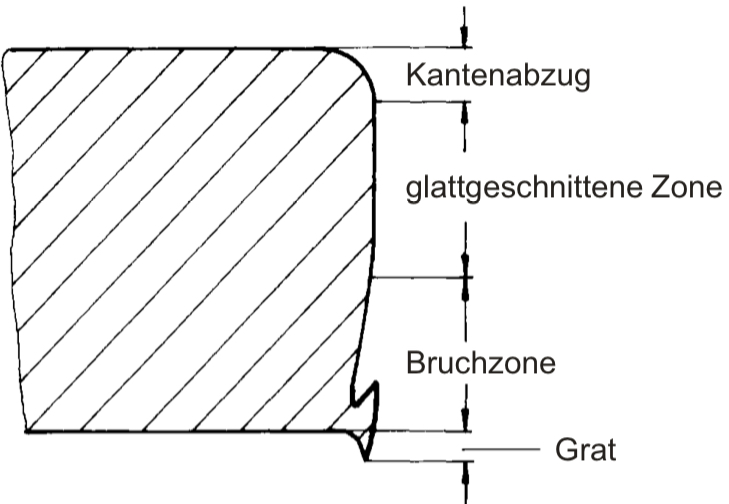
\includegraphics[width=0.8\linewidth]{src/images/Stanzen.jpeg}\\
\textbf{Verfahren:}\\
Aufsetzen des Stempels auf dem Blech, Plasitsche Verformung des
Werkstoffs, Rissbildung, Durchreissen.\\

\textbf{Feinschneiden:}\\
Beim Feinschneiden wird das Blech besonders gut eingespannt, 
sodass die Schnittkante rechtwinklig zur Planfläche des Werkstücks 
liegt.\\
Vorteile: hoher Rationalisierungsgrad, minimaler Kanterverzugs, glatte und abrissfreie Schnittfläche.\\
Schmale Rand- und Stegbreiten sind möglich. Fürs Feinschneiden ist eine gewisse Rauheit der Oberflächen nötig, um viel Reibung und genügend Halt zu gewährleisten. \\

\textbf{Masse:}\\
Beim Lochen (Innenformen) ist der Lochstempel bestimmend 
und erhält das Sollmass der Schnittteils.\\
Beim Ausschneiden 
(Aussenformen) ist der Scheidplattendurchbruch bestimmend und 
erhält das Sollmass des Schnittteils.\\
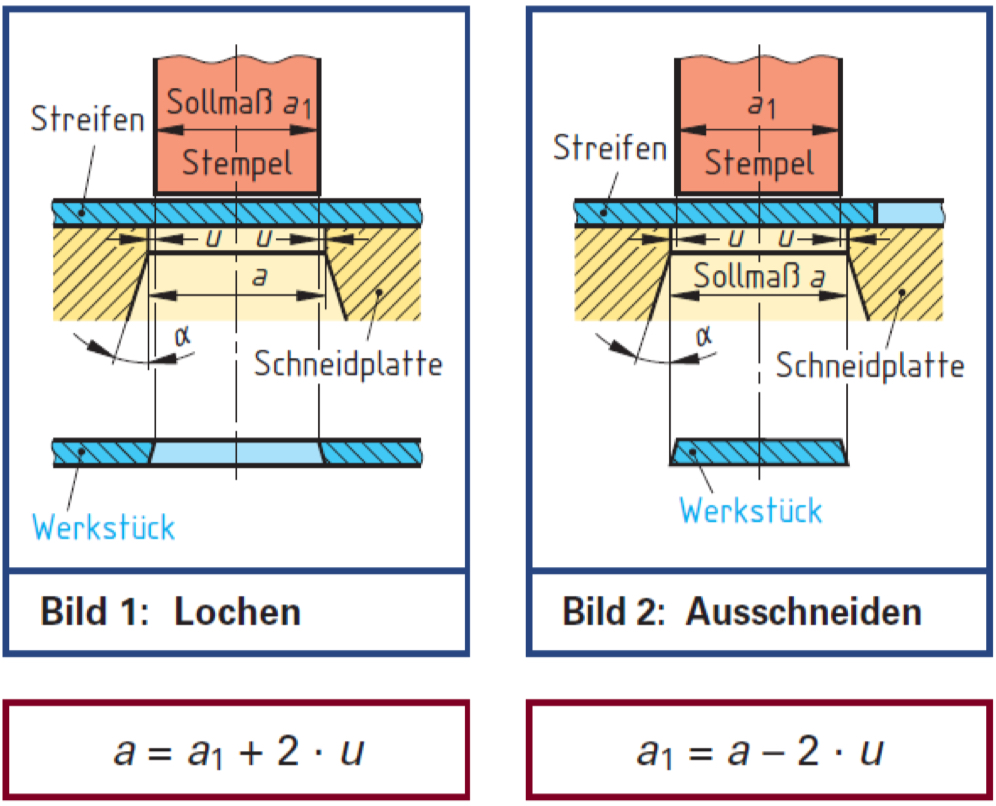
\includegraphics[width=\linewidth]{src/images/Masse Stanzen.jpeg}
